\documentclass[mathserif]{beamer}

\setbeamertemplate{frametitle}[default][center]%Centers the frame title.
\setbeamertemplate{navigation symbols}{}%Removes navigation symbols.
\setbeamertemplate{footline}{\raisebox{5pt}{\makebox[\paperwidth]{\hfill\makebox[10pt]{\scriptsize\insertframenumber}}}}

\usepackage{amsmath,amssymb,amsthm,amsfonts}
\usepackage{nicefrac}
\usepackage{graphicx,array,dsfont}
\usepackage{wrapfig}
\usepackage{harvard}
\usepackage{multirow}
\citationmode{abbr}

\newcommand{\Hrule}{\rule{\linewidth}{0.2pt}}
\newcommand{\argmax}{\mathop{\mathrm{argmax}}}
\newcommand{\argmin}{\mathop{\mathrm{argmin}}}
\newcommand{\minimize}{\mathop{\mathrm{minimize}}}
\def\half{\frac{1}{2}}
\def\th{\mathrm{th}}
\def\sign{\mathrm{sign}}
\def\supp{\mathrm{supp}}
\def\E{\mathrm{E}}
\def\P{\mathrm{P}}
\def\Var{\mathrm{Var}}
\def\Cov{\mathrm{Cov}}
\def\Cor{\mathrm{Cor}}
\def\var{\mathrm{var}}
\def\cov{\mathrm{cov}}
\def\cor{\mathrm{cor}}
\def\rcor{\mathrm{rcor}}
\def\mcor{\mathrm{mcor}}
\def\mCor{\mathrm{mCor}}
\def\dCov{\mathrm{dCov}}
\def\dcov{\mathrm{dcov}}
\def\dVar{\mathrm{dVar}}
\def\dvar{\mathrm{dvar}}
\def\dCor{\mathrm{dCor}}
\def\dcor{\mathrm{dcor}}
\def\trace{\mathrm{trace}}
\def\col{\mathrm{col}}
\def\R{\mathds{R}} 
\def\cA{\mathcal{A}}
\def\cB{\mathcal{B}}
\def\cE{\mathcal{E}}
\def\cF{\mathcal{F}}
\def\cG{\mathcal{G}}
\def\cN{\mathcal{N}}
\def\hbeta{\hat{\beta}}
\def\hy{\hat{y}}
\def\red{\color[rgb]{0.8,0,0}}
\def\white{\color[rgb]{1,1,1}}
\def\blue{\color[rgb]{0,0,0.8}}
\def\green{\color[rgb]{0,0.4,0}}

\begin{document}

\title{Tree-based methods for classification and regression}
\author{Rebecca C. Steorts \\ Predictive Modeling}
\date{November 2015}

\begin{frame}
\maketitle
{\it Optional reading: ISL 4.1, 4.2, 4.4, ESL 4.1--4.3; ISL 8.1, ESL 9.2}
\end{frame} 

\begin{frame}
\frametitle{Classification}
{\red Classification} is a predictive task in which the response takes
values across discrete categories (i.e., not continuous), and in the 
most fundamental case, two categories

\bigskip
Examples:
\begin{itemize}
\item Predicting whether a patient will develop breast cancer or remain
healthy, given genetic information
\item Predicting whether or not a user will like a new product, based on
user covariates and a history of his/her previous ratings
\item Predicting the region of Italy in which a brand of olive oil was 
made, based on its chemical composition
\item Predicting the next elected president, based on various social,
political, and historical measurements
\end{itemize}
\end{frame}

\begin{frame}
\frametitle{}
Similar to our usual setup, we observe pairs $(x_i,y_i)$, $i=1,\ldots n$, 
where $y_i$ gives the class of the $i$th observation, and $x_i \in \R^p$ are
the measurements of $p$ predictor variables

\bigskip
Though the class labels may actually be $y_i \in \{\mathrm{healthy}, 
\mathrm{sick}\}$ or $y_i \in \{\mathrm{Sardinia}, \mathrm{Sicily}, ... \}$, 
but we can always encode them as 
$$y_i \in \{1,2,\ldots K\}$$
where $K$ is the total number of classes

\bigskip
\begin{itemize}
\item Note that there is a {\red big difference} between classification and
clustering; in the latter, 
\item there is not a pre-defined notion of class 
membership (and sometimes, not even $K$), 
\item and we are not given labeled 
examples $(x_i,y_i)$, $i=1,\ldots n$, but only $x_i$, $i=1,\ldots n$
\end{itemize}
\end{frame}

\begin{frame}
\frametitle{}
\begin{itemize}
\item Assume training data $(x_i,y_i)$, $i=1,\ldots n$, 
\item Denote
classification rule by $\hat{f}(x)$; given any $x \in \R^p$, 
\item This returns a 
class label $\hat{f}(x) \in \{1,\ldots K\}$
\end{itemize}

\bigskip
As before, we will see that there are two different ways of assessing the quality 
of $\hat{f}$: its {\red predictive ability} and {\red interpretative ability}

\bigskip
\begin{tabular}{cc}
\parbox{0.5\textwidth}{
E.g., train on $(x_i,y_i)$, $i=1,\ldots n$, the data of elected presidents
and related feature measurements $x_i \in \R^p$ for the past $n$ elections,
and predict, given the current feature measurements $x_0 \in \R^p$, the winner 
of the current election}&
\hspace{3pt}
\parbox{0.35\textwidth}{
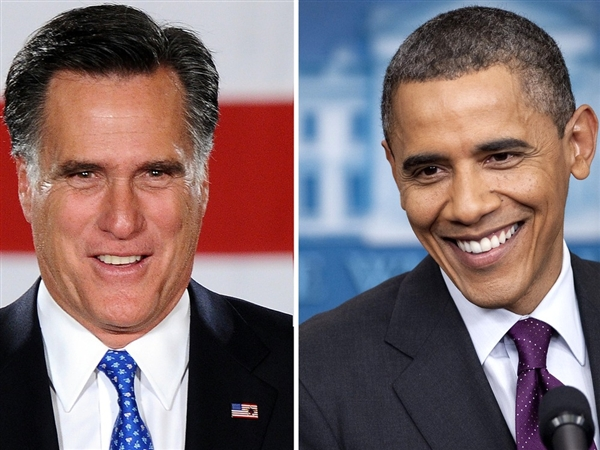
\includegraphics[width=0.35\textwidth]{candidates.jpg}
}
\end{tabular}

\bigskip
In what situations would we care more about prediction error? And in what 
situations more about interpretation?
\end{frame}

\begin{frame}
\frametitle{Binary classification and linear regression}
Let's start off by supposing that $K=2$, so that the response is 
$y_i \in \{1,2\}$, for $i=1,\ldots n$

\bigskip
You already know a tool that you could potentially use in this case for classification:
{\red linear regression}. Simply treat the response
as if it were continuous, and find the linear regression coefficients 
of the response vector $y \in \R^n$ onto the predictors, i.e., 
$$\hbeta_0, \hbeta = \argmin_{\beta_0\in\R, \,\beta \in \R^p} \, 
\sum_{i=1}^n (y_i - \beta_0 - x_i^T \beta)^2 $$

Then, given a new input $x_0 \in \R^p$, we predict the class to be
$$\hat{f}^\mathrm{LS}(x_0) = \begin{cases}
1 & \mathrm{if}\; \hbeta_0 + x_0^T \hbeta \leq 1.5 \\
2 & \mathrm{if}\; \hbeta_0 + x_0^T \hbeta  > 1.5
\end{cases}$$
\end{frame}

\begin{frame}
\frametitle{}
(Note: since we included an intercept term in the regression, it doesn't
matter whether we code the class labels as $\{1,2\}$ or $\{0,1\}$, etc.)

\bigskip
In many instances, this actually works reasonably well. Examples:

\bigskip
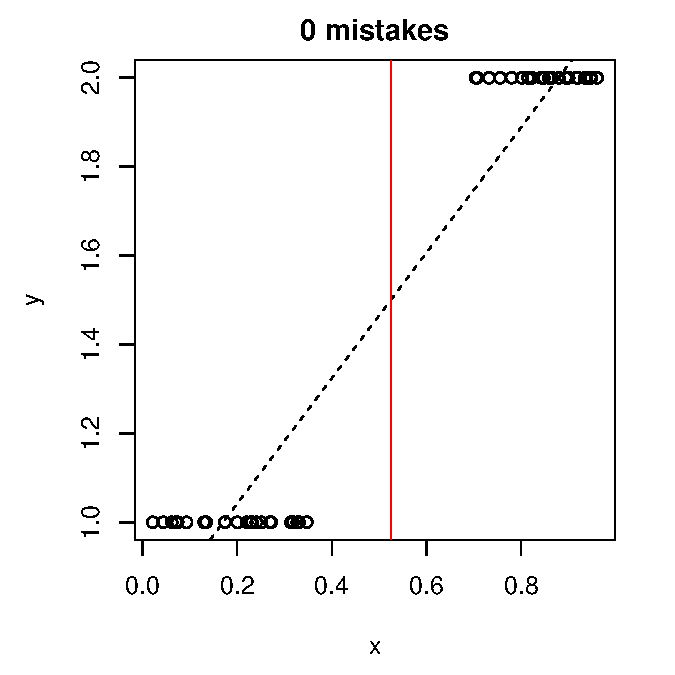
\includegraphics[width=0.33\textwidth]{lin1.pdf}
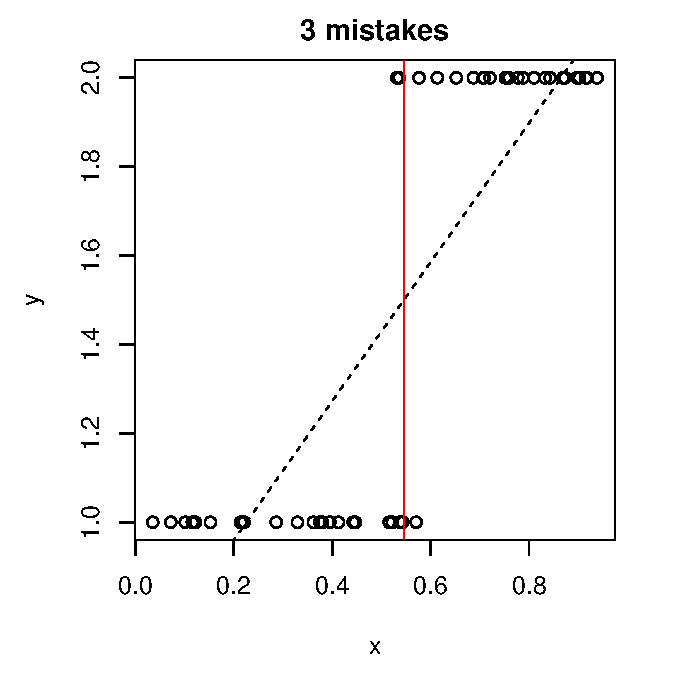
\includegraphics[width=0.33\textwidth]{lin2.pdf}
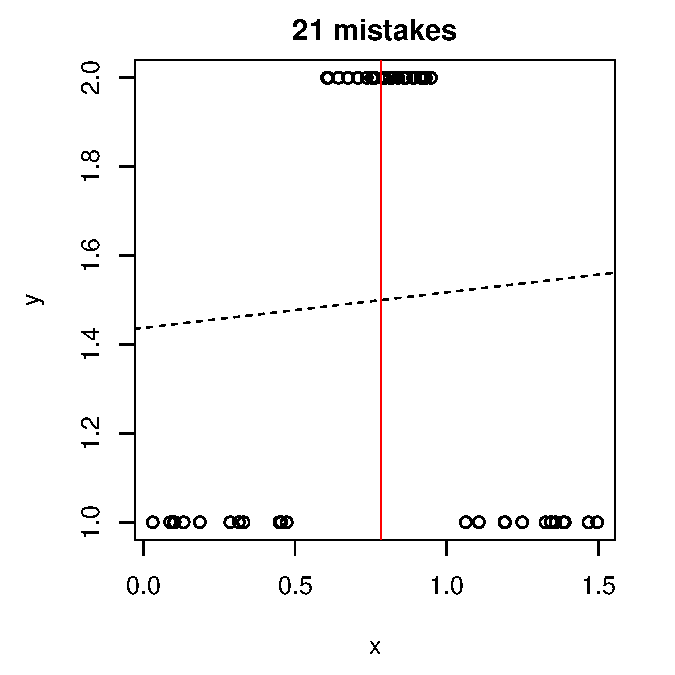
\includegraphics[width=0.33\textwidth]{lin3.pdf}
%For the last example, there is a split that achieves only 12 mistakes

\bigskip
Overall, using linear regression in this way for binary classification is not 
a crazy idea. But how about if there are more than 2 classes?
\end{frame}

\begin{frame}
\frametitle{Linear regression of indicators}
This idea extends to the case of more than two classes. Given $K$ classes,
define the {\red indicator matrix} $Y \in \R^{n\times K}$ to be the matrix
whose columns indicate class membership; that is, its $j$th column satisfies
$Y_{ij} = 1$ if $y_i=j$ (observation $i$ is in class $j$) and $Y_{ij}=0$ 
otherwise

\bigskip
E.g., with $n=6$ observations and $K=3$ classes, the matrix 
$$Y = 
\left(\begin{array}{ccc}
1 & 0 & 0 \\
1 & 0 & 0 \\
0 & 1 & 0 \\
0 & 1 & 0 \\
0 & 0 & 1 \\
0 & 0 & 1 \\
\end{array}\right) \in \R^{6 \times 3}$$
corresponds to having the first two observations in class 1, the next two
in class 2, and the final 2 in class 3
\end{frame}

\begin{frame}
\frametitle{}
To construct a prediction rule, we regress 
each column $Y_j \in \R^n$ (indicating the $j$th class versus all else)
onto the predictors:
$$\hbeta_{j,0}, \hbeta_j = \argmin_{\beta_{j,0}\in\R,\,\beta_j \in \R^p} 
\, \sum_{i=1}^n (Y_{ij} - \beta_{0,j} - \beta_j^T x_i)^2$$

Now, given a new input $x_0 \in \R^p$, we compute
$$\hbeta_{0,j} + x_0^T \hbeta_j, \;\;\; j=1,\ldots K$$
take predict the class $j$ that corresponds to the highest score. I.e., we let
each of the $K$ linear models {\red make its own prediction}, and then we take 
the strongest. Formally, $$\hat{f}^\mathrm{LS}(x_0) = 
\argmax_{j=1,\ldots K} \; \hbeta_{0,j} + x_0^T \hbeta_j $$
\end{frame}

\begin{frame}
\frametitle{}
The {\red decision boundary} between any two classes $j,k$ are the values of
$x \in \R^p$ for which 
$$\hbeta_{0,j} + x^T \hbeta_j  = \hbeta_{0,k} + x^T \hbeta_k$$
i.e., $\hbeta_{0,j}-\hbeta_{0,k} + (\hbeta_j-\hbeta_k)^T x = 0$

\bigskip
\bigskip
\begin{tabular}{cc}
\parbox{0.475\textwidth}{

\includegraphics[width=0.475\textwidth]{blank.png}}
%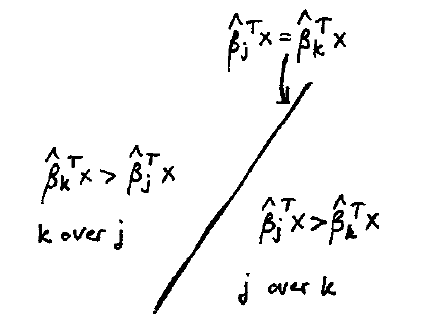
\includegraphics[width=0.475\textwidth]{db.png}}
\hspace{-15pt}
\parbox{0.5\textwidth}{
This defines a $(p-1)$-dimensional affine subspace in $\R^p$. 
% it's actually affine if we include intercept
To one side, we would always predict class $j$
over $k$; to the other, we would always predict class $k$ over $j$}
\end{tabular}

\bigskip
\bigskip
\bigskip
For $K$ classes total, there are ${K \choose 2}=\frac{K(K-1)}{2}$ decision boundaries
\end{frame}

\begin{frame}
\frametitle{Ideal result}
\smallskip
What we'd like to see when we use linear regression for a
3-way classification (from ESL page 105):
\vspace{-2pt}
\begin{center}
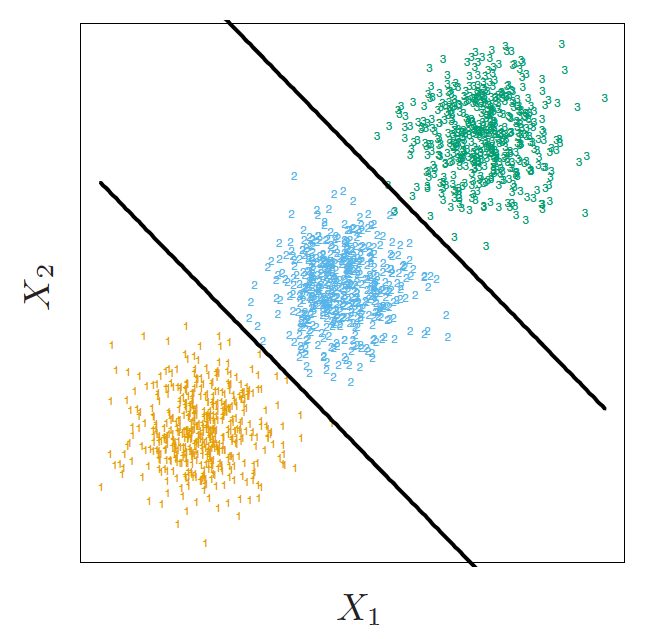
\includegraphics[width=2.25in]{ideal.png}
\end{center}
\vspace{-5pt}
The plotted lines are the decision boundaries between classes 1 and 2, and 2 and 3
(the decision boundary between classes 1 and 3 never matters)
\end{frame}

\begin{frame}
\frametitle{Actual result}
\smallskip
What actually happens when we use linear regression for this 3-way classification
(from ESL page 105):
\begin{center}
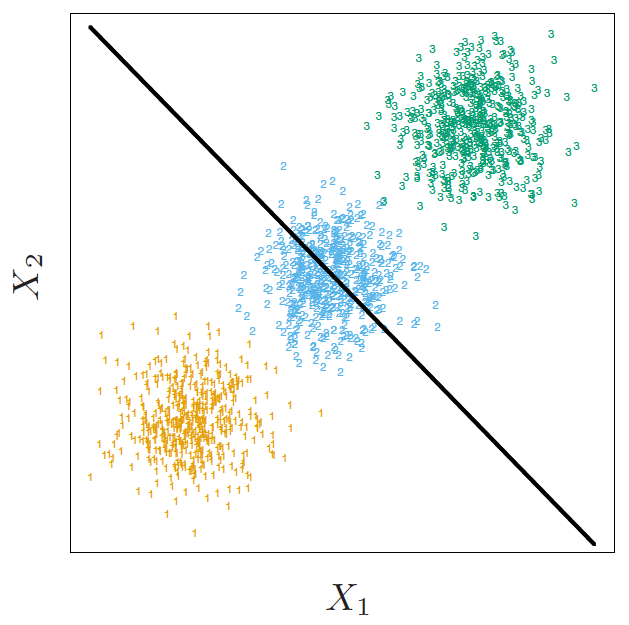
\includegraphics[width=2.20in]{actual.png}
\end{center}
\vspace{-5pt}
The decision boundaries between 1 and 2 and between 2 and 3 are the same, so we 
would never predict class 2. This problem is called {\red masking} (and it is not
uncommon for moderate $K$ and small $p$)
\end{frame}

\begin{frame}
\frametitle{Why did this happen?}
Projecting onto the line joining the three class centroids gives some insight into 
why this happened (from ESL page 106):
\begin{center}
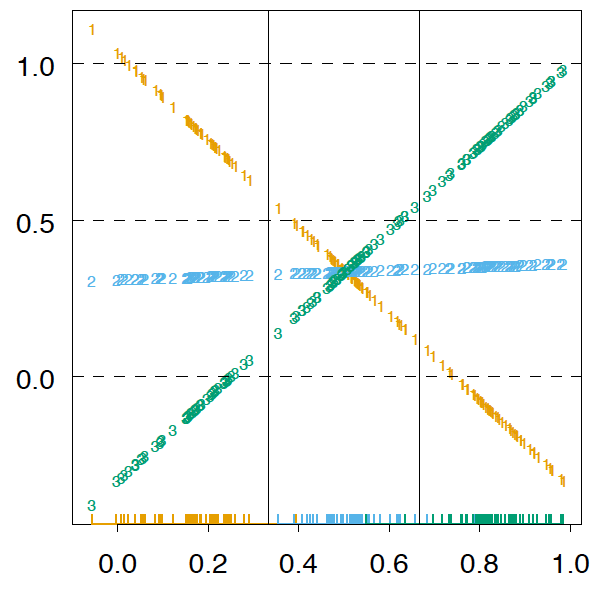
\includegraphics[width=2.6in]{why.png}
\end{center}
\end{frame}

\begin{frame}
\frametitle{Methods I'm not covering}
\begin{itemize}
\item LDA and QDA
\item logistic versions
\item See ISL to learn more
\end{itemize}
\end{frame}


\begin{frame}
\frametitle{Tree-based methods}
{\red Tree-based based} methods for predicting $y$ from a feature
vector $x \in \R^p$ divide up the feature space into rectangles,
and then fit a very simple model in each rectangle. This works
both when $y$ is discrete and continuous, i.e., both for 
{\red classification} and {\red regression}

\bigskip
Rectangles can be achieved by making successive 
binary splits on the predictors variables $X_1,\ldots X_p$. I.e.,
we choose a variable $X_j$, $j=1,\ldots p$, {\red divide} up the 
feature space according to 
$$X_j \leq c \;\;\;\text{and}\;\;\; X_j > c$$ Then we proceed
on each half

\bigskip For simplicity, consider classification first
(regression later). If a half is ``pure'', meaning that it
mostly contains points from one class, then we
don't need to continue splitting; otherwise, we continue splitting
\end{frame}

\begin{frame}
\frametitle{Example: simple classification tree}
Example: $n=500$ points in $p=2$ dimensions, falling into classes 
0 and 1, as marked by colors

\smallskip
\begin{center}
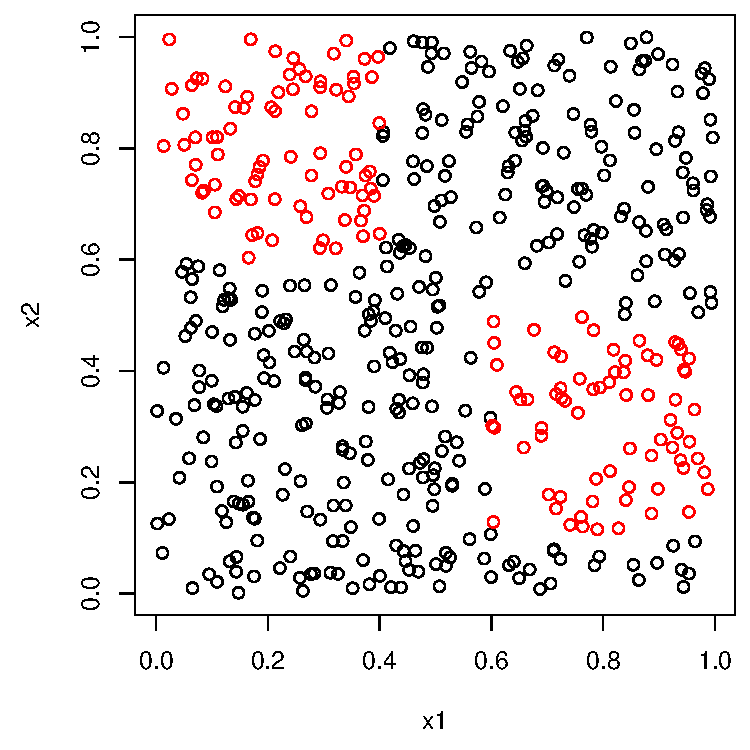
\includegraphics[width=2in]{simpledata.pdf}
\end{center}

\vspace{-4pt}
Does dividing up the feature space into rectangles look like it
would work here?
\end{frame}

\begin{frame}
\frametitle{}
\bigskip
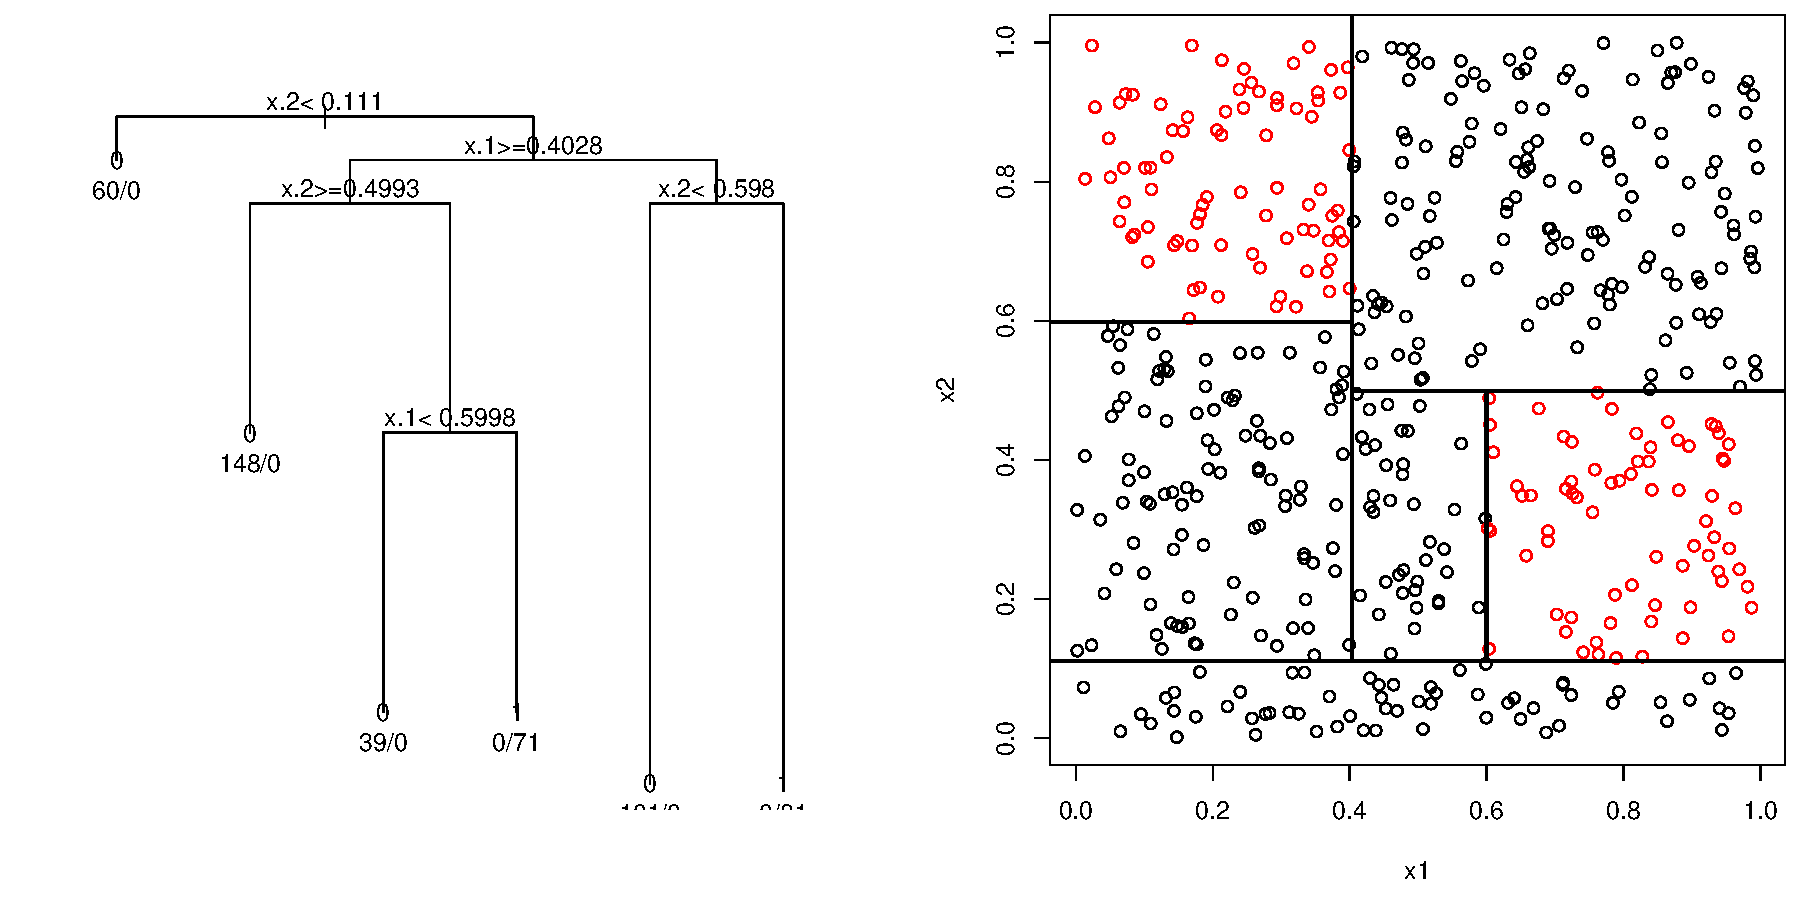
\includegraphics[width=\textwidth]{simpletree.pdf}
\end{frame}

%\begin{frame}
%\frametitle{Example: HCV treatment flow chart}
%\smallskip
%\begin{center}
%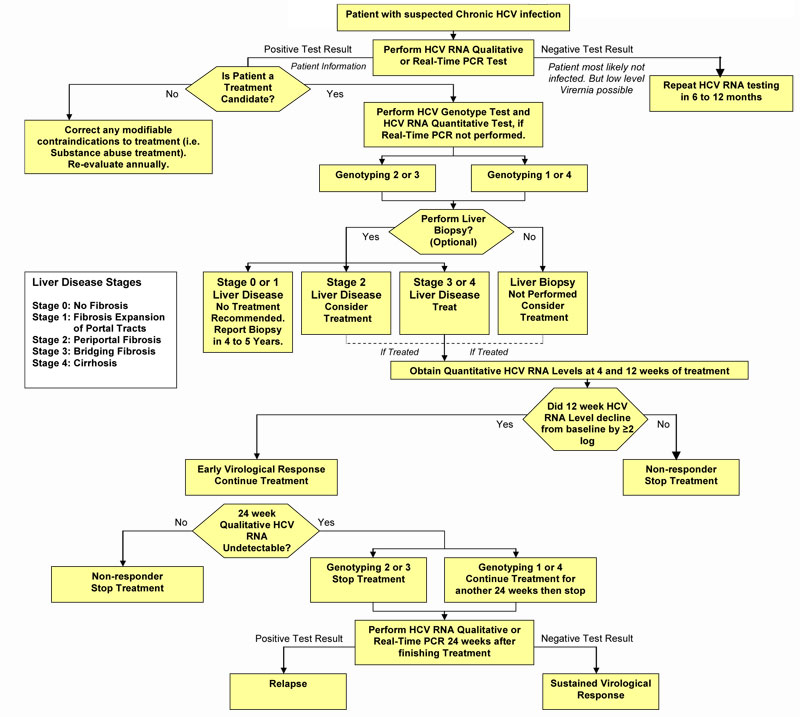
\includegraphics[width=0.75\textwidth]{flowchart.jpg}
%\end{center}
%(From {\footnotesize \url{http://hcv.org.nz/wordpress/?tag=treatment-flow-chart}})
%\end{frame}

\begin{frame}
\frametitle{Classification trees}
\smallskip
{\red Classification trees} are popular because they are 
interpretable, and maybe also because they mimic the way (some) decisions 
are made

\bigskip
Let $(x_i,y_i)$, $i=1,\ldots n$ be the training data, where 
$y_i \in \{1,\ldots K\}$ are the class labels, and 
$x_i \in \R^p$
measure the $p$ predictor variables. The classification tree can
be thought of as defining $m$ regions (rectangles) $R_1,\ldots R_m$, each 
corresponding to a leaf of the tree

\bigskip
We assign each $R_j$ a class label $c_j \in \{1,\ldots K\}$. We then 
classify a new point $x \in \R^p$ by
$$\hat{f}^\mathrm{tree}(x) \;=\; \sum_{j=1}^m c_j \cdot 1\{x \in R_j\}
\;=\; c_j \;\, \mathrm{such}\;\mathrm{that}\;\, x \in R_j$$
Finding out which region a given point $x$ belongs to is {\red easy} since
the regions $R_j$ are defined by a tree---we just scan down the tree.
Otherwise, it would be a lot harder (need to look at each region)
\end{frame}

\begin{frame}
\frametitle{Example: regions defined by a tree}
\bigskip
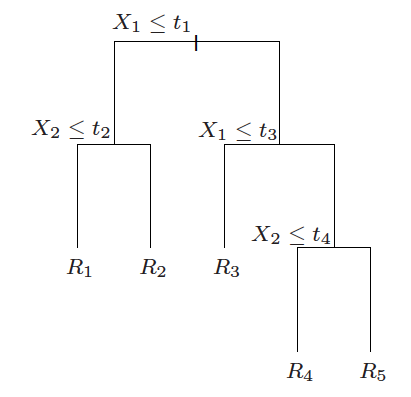
\includegraphics[width=2.2in]{ex1-tree.png}
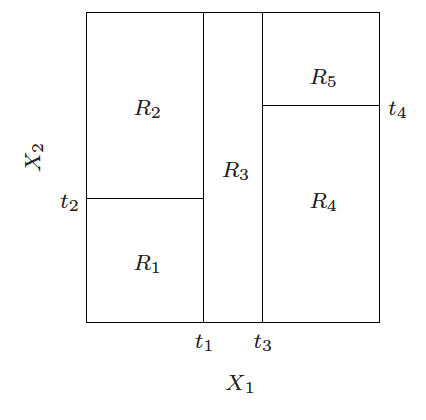
\includegraphics[width=2.2in]{ex1-regions.png}

\bigskip
(From ESL page 306)
\end{frame}

\begin{frame}
\frametitle{Example: regions not defined a tree}
\begin{center}
\bigskip
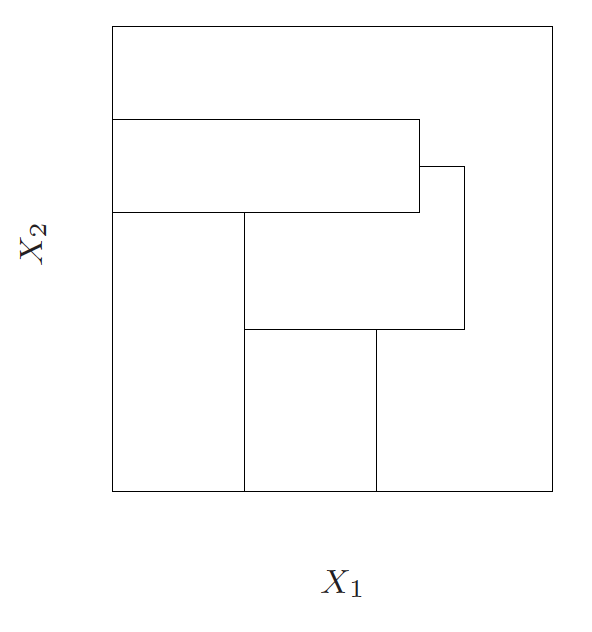
\includegraphics[width=2.5in]{ex1-notpos.png}
\end{center}
\vspace{-5pt}
(From ESL page 306)
\end{frame}

\begin{frame}
\frametitle{Predicted class probabilities}
\smallskip
\smallskip
With classification trees, we can also get not only the predicted
classes for new points but also the {\red predicted class probabilties}

\bigskip
Note that each region $R_j$ contains some subset of the training data
$(x_i,y_i)$, $i=1,\ldots n$, say, $n_j$ points. The predicted class $c_j$ is 
just most common occuring class among these points. Further, for each class
$k=1,\ldots K$, we can estimate the probability that the class label is $k$
given that the feature vector lies in region $R_j$, $\P(C=k|X\in R_j)$, by
$$\hat{p}_k (R_j) = \frac{1}{n_j}\sum_{x_i \in R_j} 1\{y_i = k\}$$
the {\red proportion of points} in the region that are of class $k$. 
We can now express the predicted class as
$$c_j = \argmax_{k=1,\ldots K} \; \hat{p}_k (R_j)$$
\end{frame}

\begin{frame}
\frametitle{Trees provide a good balance}
\begin{center}
\begin{tabular}{|c|c|c|c|c|}
\hline
& \parbox{0.8in}{\centering Model \\ assumptions?} &
\parbox{0.8in}{\centering Estimated \\ probabilities?} &
Interpretable? & Flexible? \\
\hline
LDA & Yes & Yes & Yes & No \\
\hline
LR & Yes & Yes & Yes & No \\
\hline
$k$-NN & No & No & No & Yes \\
\hline
Trees & No & Yes & Yes & Somewhat \\
\hline
\end{tabular}

\bigskip
\bigskip
\begin{tabular}{|c|c|}
\hline
& \parbox{1in}{\centering Predicts \\ well?} \\
\hline
LDA & Depends on $X$ \\
\hline
LR & Depends on $X$ \\
\hline
$k$-NN & \parbox{1in}{\centering If properly \\ tuned} \\
\hline
Trees & ? \\
\hline
\end{tabular}
\end{center}

%% \smallskip
%% Remember that for both {\red LDA} and {\red logistic regression} we were able 
%% to estimate the class probabilities $P(C=j|X=x)$; for LDA we did this by
%% assuming that $X|C=j$ had a Gaussian distribution, for logistic regression
%% we did this by assuming that the log odds was linear in $x$. These methods
%% were also nice in that they could (potentially) give insight into the relationship 
%% between $X$ and $C$.

%% \bigskip
%% For the {\red model-free} classification methods, by $k$-nearest-neighbors 
%% and $K$-means clustering, there wasn't obvious way to estimate the class
%% probabilities. (You could think of a way to do this for large numbers
%% of neighbors of large numbers of centroids---but still, these wouldn't
%% be great.) The methods were also not interpretable.

%% \bigskip
%% Trees provide a nice {\red balance} between the two types of rules
%% above. They don't make any model assumptions, but still are highly interpretable 
%% and give estimated class probabilities. Their decision boundaries (rectangles) aren't 
%% as flexible as those for $k$-nearest- neighbors or $K$-means clustering, but are
%% still pretty general.
\end{frame}

\begin{frame}
\frametitle{How to build trees?}

\smallskip
There are two main issues to consider in building a tree:
\begin{enumerate}
\item How to choose the splits?
\item How big to grow the tree?
\end{enumerate}

\bigskip
Think first about varying the depth of the tree ... which is more complex,
a big tree or a small tree? What {\red tradeoff} is at play here? 
How might we eventually consider choosing the depth?

\bigskip
Now for a fixed depth, consider choosing the splits. If the tree has 
depth $d$ (and is balanced), then it has $\approx 2^d$ nodes. At each node
we could choose any of $p$ the variables for the split---this means 
that the number of possibilities is
\vspace{-3pt}
$$p \cdot 2^d
\vspace{-3pt}$$
This is {\red huge} even for moderate $d$! And we haven't even
counted the actual split points themselves
\end{frame}

\begin{frame}
\frametitle{The CART algorithm}
\smallskip
The {\red CART algorithm}\footnote{Breiman et al. (1984), ``Classification
and Regression Trees''} 
chooses the splits in a top down fashion: then chooses the first variable 
to at the root, then the variables at the second level, etc. 

\bigskip
At each stage we choose the split to achieve the biggest
drop in misclassification error---this is called a {\red greedy} strategy.
In terms of tree depth, the strategy is to grow a large tree and then {\red prune} 
at the end

%\smallskip
%\smallskip
%\begin{tabular}{cc}
%\parbox{0.5\textwidth}{
%Why grow a large tree and prune, instead of just stopping at some point?
%Because any stopping rule may be {\red short-sighted}, in that a split
%may look bad but it may lead to a good split below it} &
%\parbox{0.4\textwidth}{
%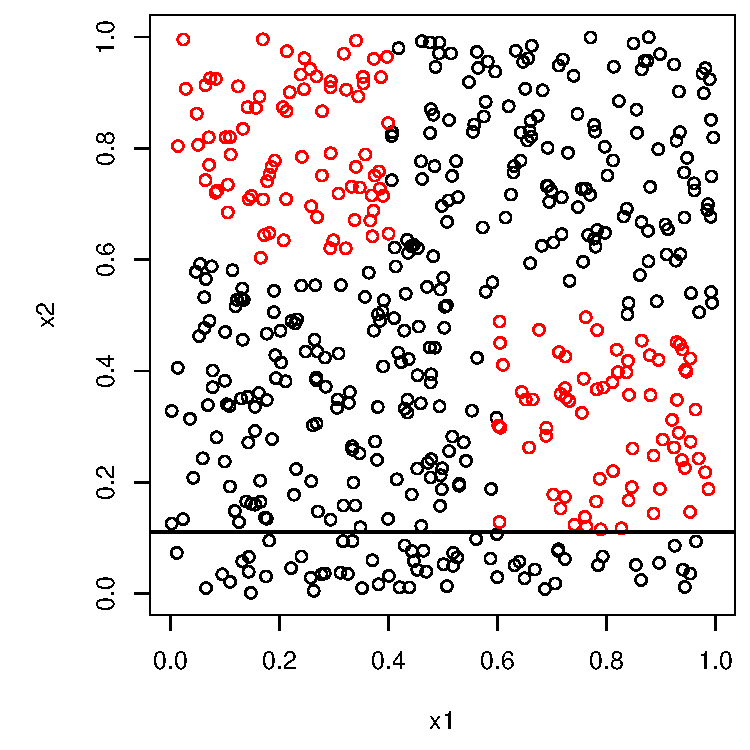
\includegraphics[width=0.4\textwidth]{stop.pdf}}
%\end{tabular}
\end{frame}

\begin{frame}
\frametitle{}
Recall that in a region $R_m$, the proportion of points in class $k$ is
$$\hat{p}_k(R_m) = \frac{1}{n_m} \sum_{x_i \in R_m} 1\{y_i=k\}.$$
The CART algorithm begins by considering splitting on variable $j$ and split 
point $s$, and defines the regions
$$R_1 = \{X \in \R^p : X_j \leq s\}, \;\;
R_2 = \{X \in \R^p : X_j > s\}$$
We then {\red greedily} chooses $j,s$ by minimizing the misclassification error
$$\argmin_{j,s} \; \Big( \big[1-\hat{p}_{c_1}(R_1)\big] + 
\big[1-\hat{p}_{c_2}(R_2)\big] \Big)$$
Here $c_1 = \argmax_{k=1,\ldots K} \, \hat{p}_k(R_1)$ is the most common class
in $R_1$, and $c_2 = \argmax_{k=1,\ldots K} \, \hat{p}_k(R_2)$ is the most 
common class in $R_2$
\end{frame}

\begin{frame}
\frametitle{}
\smallskip
\bigskip
Having done this, we now repeat this within each of the newly defined
regions $R_1,R_2$. That is, it again considers splitting all variables $j$ and
split points $s$,  within each of $R_1,R_2$, this time greedily choosing the pair 
that provides us with the biggest {\red improvement} in misclassification error

\bigskip
How do we find the best split $s$? Aren't there {\red infinitely many} to consider?
No, to split a region $R_m$ on a variable $j$, we really only need to consider $n_m$ 
splits (or $n_m-1$ splits)

\smallskip
\begin{center}
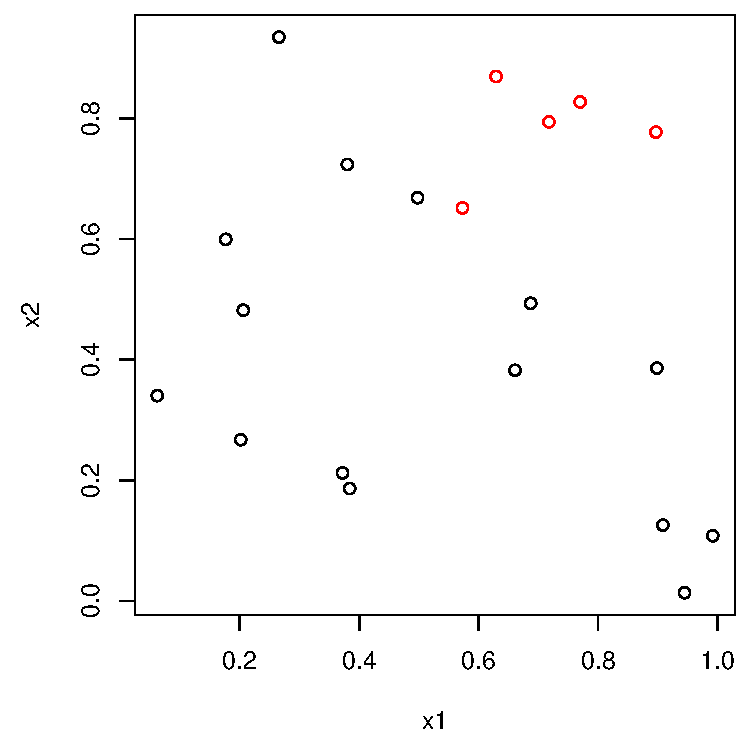
\includegraphics[width=1.5in]{split1.pdf}
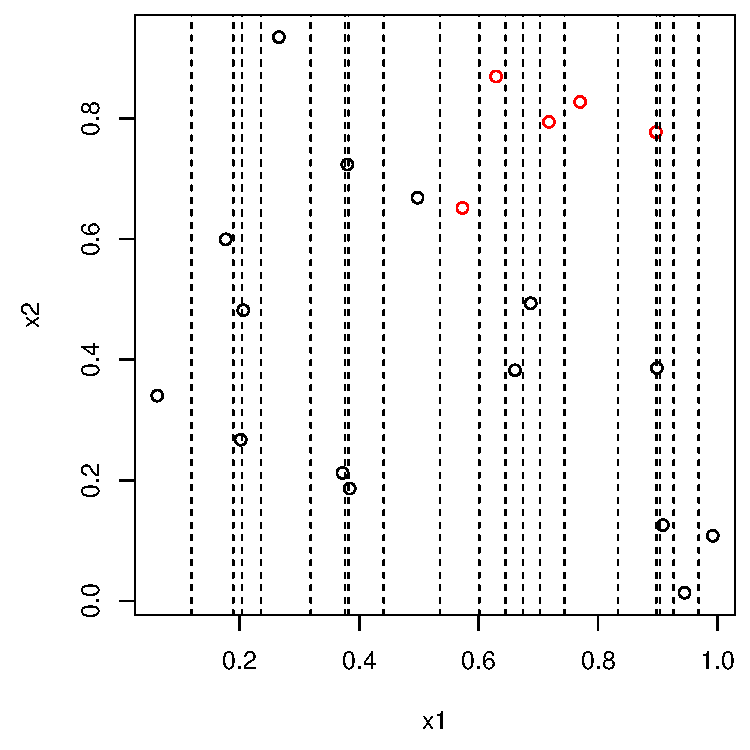
\includegraphics[width=1.5in]{split2.pdf}
\end{center}
\end{frame}

\begin{frame}
\frametitle{}
\bigskip
\begin{tabular}{cc}
\parbox{0.35\textwidth}{
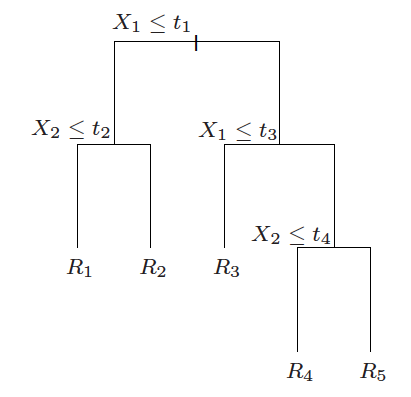
\includegraphics[width=0.35\textwidth]{ex1-tree.png}} &
\hspace{3pt}
\parbox{0.5\textwidth}{
Continuing on in this manner, we will get a big tree $T_0$. Its leaves define regions
$R_1,\ldots R_m$. We then {\red prune} this tree, meaning that we collapse some of its 
leaves into the parent nodes}
\end{tabular}

\smallskip
\smallskip
For any tree $T$, let $|T|$ denote its number of leaves.
We define
\vspace{-3pt}
$$C_\alpha(T) = \sum_{j=1}^{|T|} \big[1-\hat{p}_{c_j}(R_j)\big] + \alpha|T|
\vspace{-3pt}$$
We seek the tree $T \subseteq T_0$ that minimizes $C_\alpha(T)$. It turns out that 
this can be done by pruning the weakest leaf one at a time. Note that $\alpha$ is 
a {\red tuning parameter}, and a larger $\alpha$ yields a smaller tree.
CART picks $\alpha$ by 5- or 10-fold cross-validation
\end{frame}

\begin{frame}
\frametitle{Example: simple classification tree}
\smallskip
Example: $n=500$, $p=2$, and $K=2$. We ran CART:

\smallskip
\smallskip
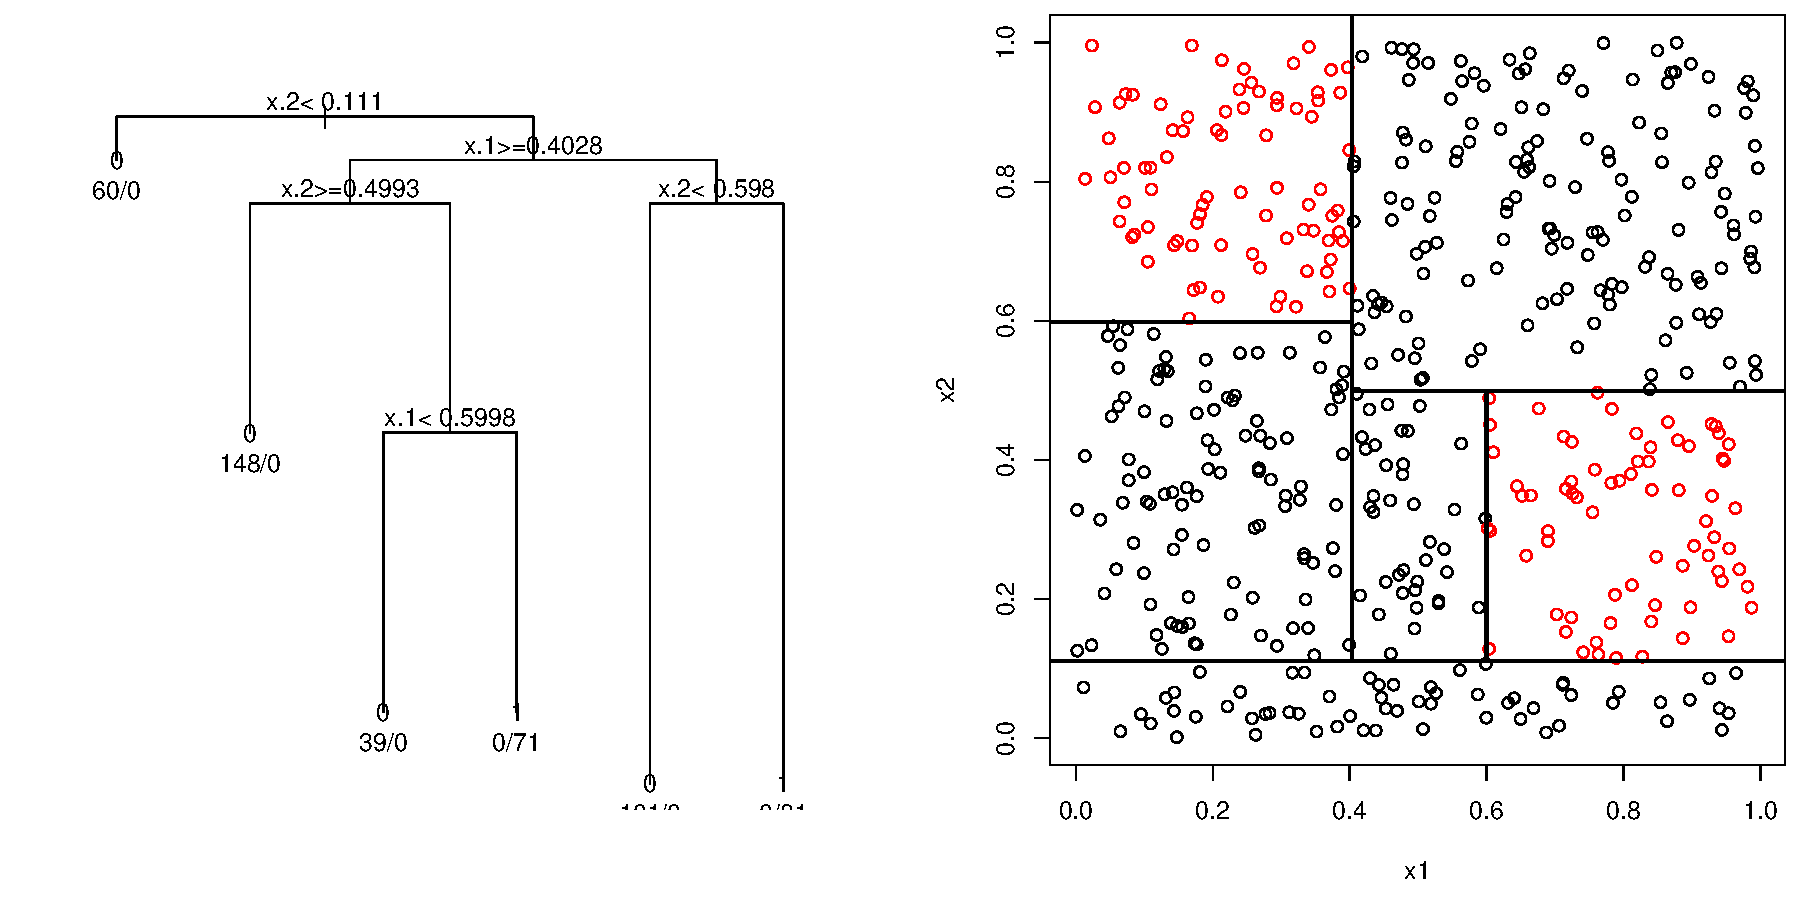
\includegraphics[width=\textwidth]{simpletree.pdf}

\smallskip
\smallskip
To use CART in R, you can use either of the functions {\tt rpart} or {\tt tree}, in the 
packages of those same names.
When you call {\tt rpart}, cross-validation is performed automatically; 
when you call {\tt tree}, you must then call {\tt cv.tree} for cross-validation
\end{frame}

\begin{frame}
\frametitle{Example: spam data}
\smallskip
Example: $n=4601$ emails, of which 1813 are considered spam. For each email
we have $p=58$ attributes. The first 54 measure the frequencies of 54 key words
or characters (e.g., ``free'', ``need'', ``\$''). The last 3 measure 
\begin{itemize}
\item the average length of uninterrupted sequences of capitals;
\item the length of the longest uninterrupted sequence of capitals;
\item the sum of lengths of uninterrupted sequences of capitals
\end{itemize}
(Data from ESL section 9.2.5)

\bigskip
An aside: how would we possibly get thousands of emails labeled as spam or not?
\begin{center}

\includegraphics[width=0.6\textwidth]{gmail.png}
\end{center}
This is great! Every time you label an email as spam, gmail has more training datafg
\end{frame}

\begin{frame}
\frametitle{}
\bigskip
Cross-validation error curve for the spam data (from ESL page 314):

\vspace{-5pt}
\begin{center}
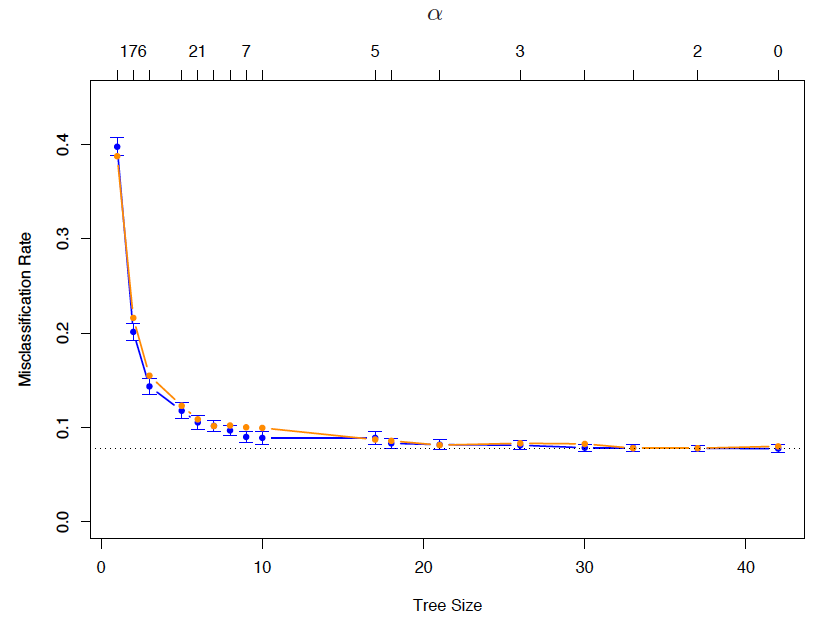
\includegraphics[width=3.5in]{spamcv.png}
\end{center}
\end{frame}

\begin{frame}
\frametitle{}
\bigskip
Tree of size 17, chosen by cross-validation (from ESL page 315):

\vspace{-5pt}
\begin{center}
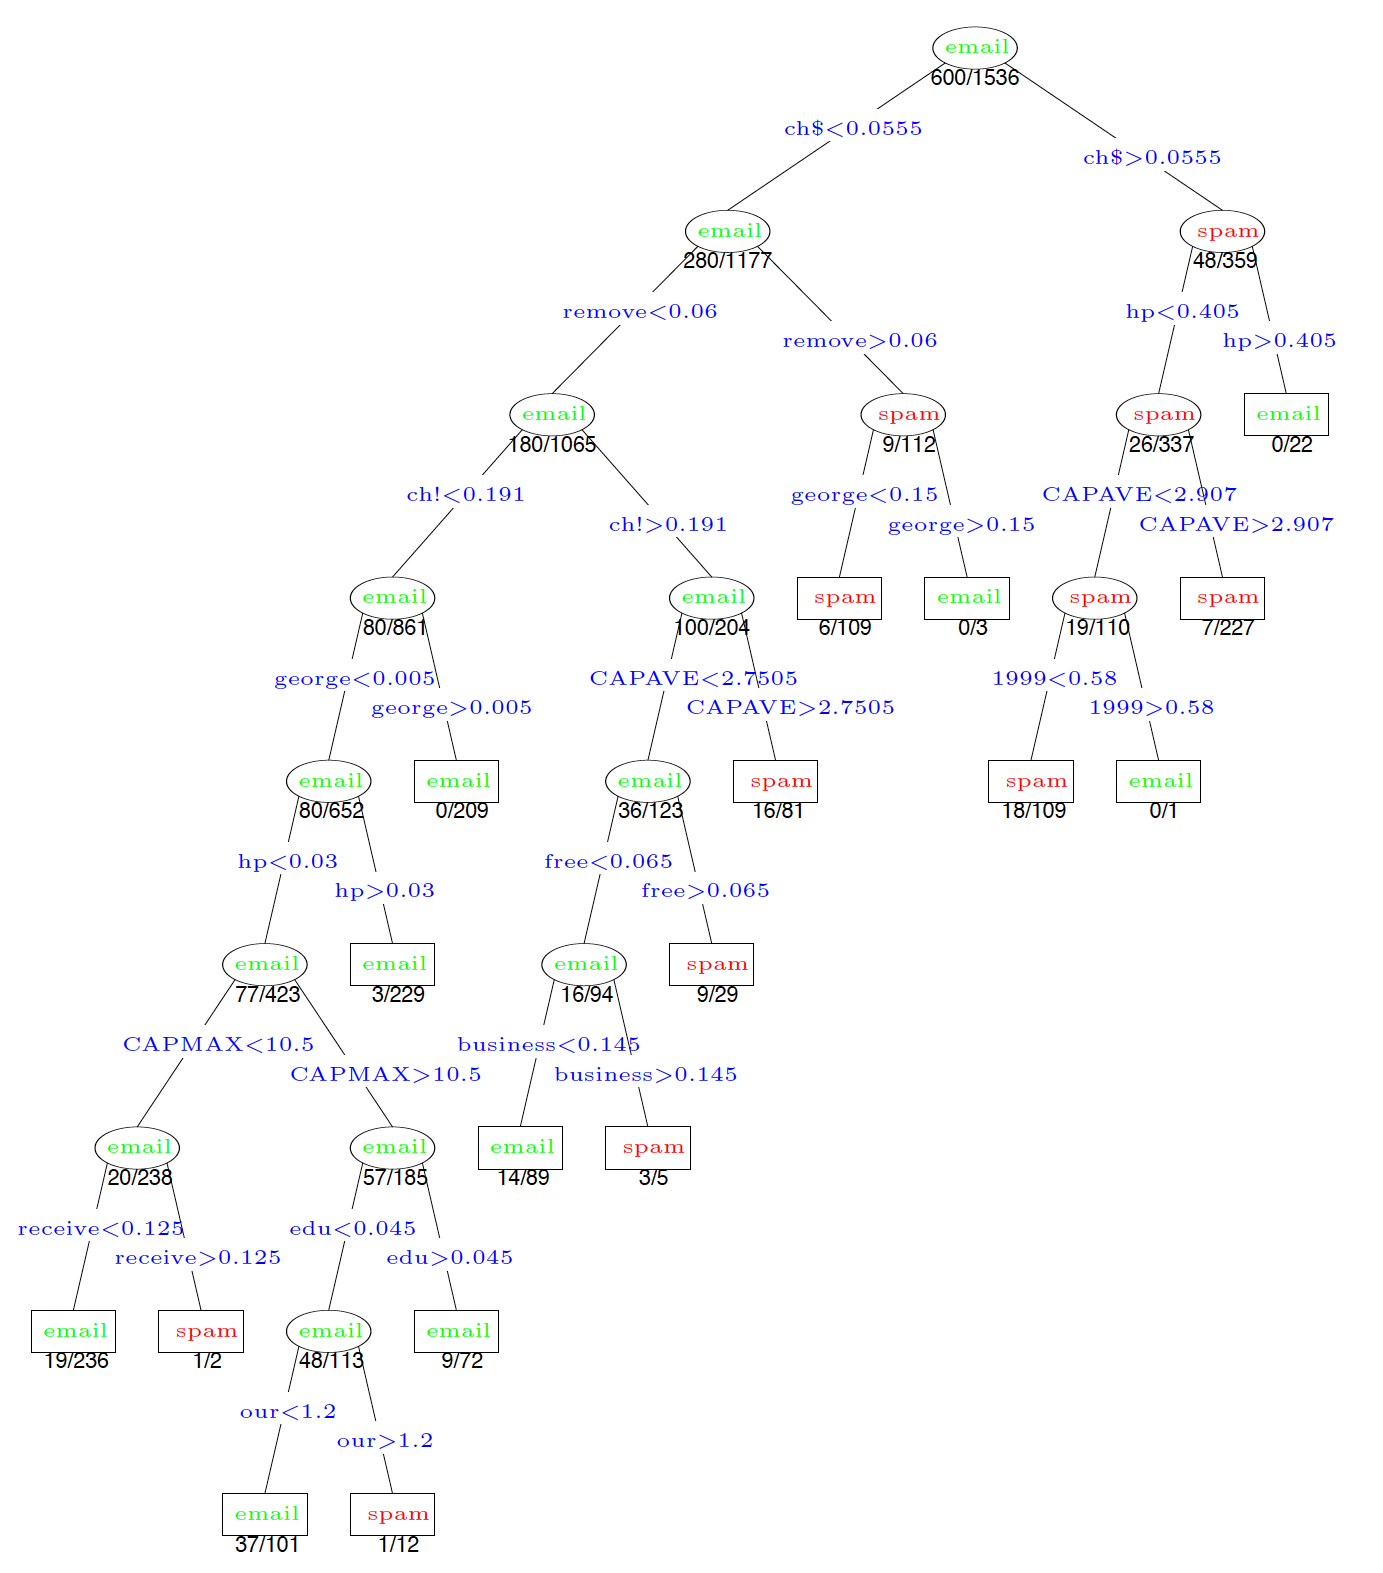
\includegraphics[width=2.7in]{spamtree.png}
\end{center}
\end{frame}

\begin{frame}
\frametitle{Other impurity measures}
We used misclassification error as a measure of the impurity of region $R_j$,
$$1-\hat{p}_{c_j}(R_j)$$
But there are other useful measures too: the {\red Gini index}:
$$\sum_{k=1}^K \hat{p}_k(R_j) \big[1-\hat{p}_k(R_j)\big],$$
and the {\red cross-entropy} or {\red deviance}:
$$-\sum_{k=1}^K \hat{p}_k(R_j) \log\big\{\hat{p}_k(R_j) \big\}.$$
Using these measures instead of misclassification error is sometimes preferable 
because they are more sensitive to changes in class probabilities. Overall, 
they are all pretty similar (Homework 7)
\end{frame}

\begin{frame}
\frametitle{Regression trees}
Suppose that now we want to predict a {\red continuous} outcome instead of a class
label. Essentially, everything follows as before, but now we just fit a constant 
inside each rectangle

\smallskip
\begin{center}
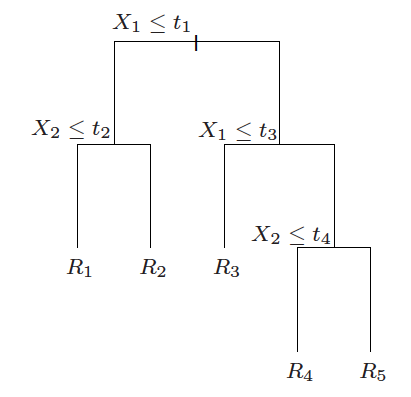
\includegraphics[width=2in]{ex1-tree.png}
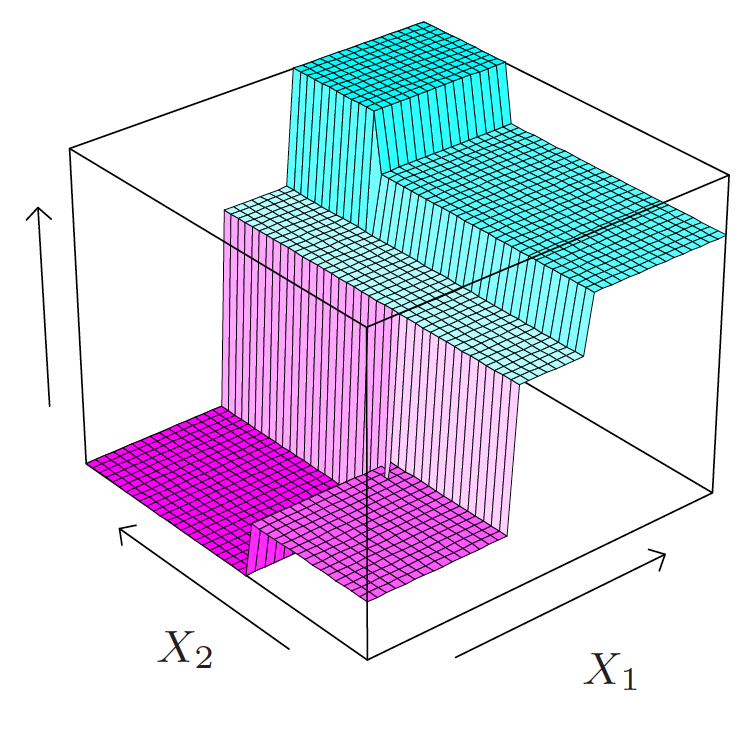
\includegraphics[width=2in]{regtree.png}
\end{center}
\end{frame}

\begin{frame}
\frametitle{}
\smallskip
The estimated regression function has the form
$$\hat{f}^\mathrm{tree}(x) \;=\; \sum_{j=1}^m c_j \cdot 1\{x \in R_j\}
\;=\; c_j \;\, \mathrm{such}\;\mathrm{that}\;\, x \in R_j$$
just as it did with classification. The quantities $c_j$ are
no longer predicted classes, but instead they are real numbers. 
How would we choose these? Simple: just take the average response of all of the
points in the region,
$$c_j = \frac{1}{n_j} \sum_{x_i \in R_j} y_i$$ 

The main difference in building the tree is that we use {\red squared error loss} 
instead of misclassification error (or Gini index or deviance) to decide which region
to split. Also, with squared error loss, choosing $c_j$ as above is optimal
\end{frame}

\begin{frame}
\frametitle{How well do trees predict?}
\smallskip
Trees seem to have a lot of things going in the favor. So how is their 
predictive ability?

\bigskip
Unfortunately, the answer is {\red not great}. Of course, at a high level, 
the prediction error is governed by bias and variance, which in turn
have some relationship with the size of the tree (number of nodes). 
A larger size means smaller bias and higher variance, and a smaller
tree means larger bias and smaller variance

\bigskip
But trees generally suffer from high variance because they are quite
{\red instable}: a smaller change in the observed data can lead to a 
dramatically different sequence of splits, and hence a different prediction.
This instability comes from their hierarchical nature; once a split is made,
it is permanent and can never be ``unmade'' further down in the tree

\bigskip
We'll learn some variations of trees have {\red much better} predictive
abilities. However, their predictions rules aren't as transparent
\end{frame}

\begin{frame}
\frametitle{Recap: trees for classification and regression}
In this lecture, we learned about {\red trees} for classification and 
regression. Using trees, we divide the feature space up into rectangles
by making successive splits on different variables, and then within
each rectangle (leaf of the tree), the predictive task is greatly 
{\red simplified}. I.e., in classification, we just predict the most
commonly occuring class, and in regression, we just take the average
response value of points in the region

\bigskip
The space of possible trees is huge, but we can fit a good tree using
a {\red greedy} strategy, as is done by the {\red CART algorithm}.
It also grows a large tree, and then prunes back at the end, choosing
how much to prune by cross-validation

\bigskip
Trees are model-free and are easy to interpret, but generally speaking,
aren't very powerful in terms of predictive ability. Next time we'll learn
some procedures that use trees to make excellent prediction engines (but
in a way we lose interpretability)
\end{frame}


\begin{frame}
\frametitle{Next time: bagging}
\smallskip
Fitting small trees on bootstrapped data sets, and averaging predictions
at the end, can greatly reduce the prediction error (from ESL page 285):

\begin{center}
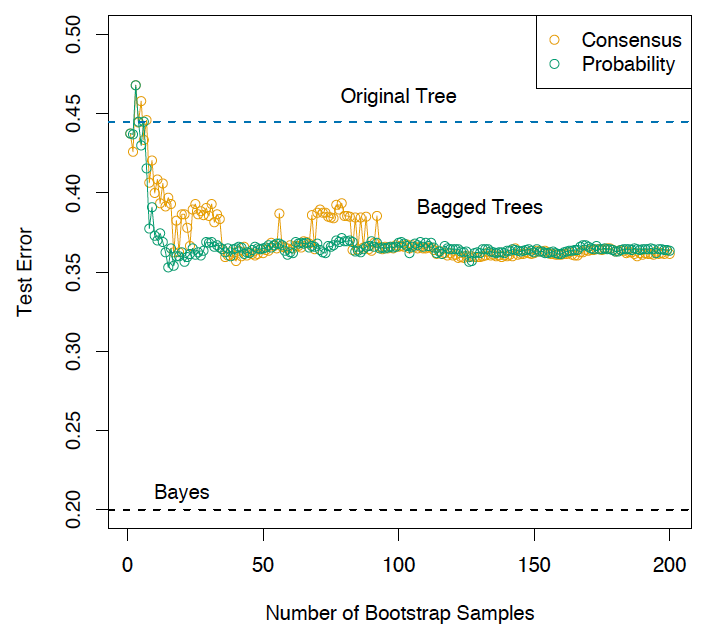
\includegraphics[width=2.5in]{bagging.png}
\end{center}
\end{frame}

\end{document}


